\documentclass[conference]{IEEEtran}

\usepackage{amsmath,amssymb,amsfonts}
\usepackage{graphicx}
\usepackage{textcomp}
\usepackage{xcolor}
\usepackage{booktabs}
\usepackage{array}
\usepackage{listings}
\usepackage{url}
\usepackage{hyperref}
\usepackage{cite}

% Code Listing Style
\lstset{
	language=Python,
	basicstyle=\ttfamily\footnotesize,
	keywordstyle=\color{blue}\bfseries,
	commentstyle=\color{gray}\itshape,
	stringstyle=\color{red},
	numbers=left,
	numberstyle=\tiny\color{gray},
	numbersep=5pt,
	frame=single,
	breaklines=true,
	captionpos=b,
	tabsize=4
}

\def\BibTeX{{\rm B\kern-.05em{\sc i\kern-.025em b}\kern-.08em
		T\kern-.1667em\lower.7ex\hbox{E}\kern-.125emX}}

\begin{document}
	
	\title{Predicting Customer Churn in the Telecommunications Industry: A Comparative Study of Classification Algorithms\\
		{\footnotesize BIL 476 --- Data Mining Course Project, Summer 2026\\
			TOBB University of Economics and Technology}
	}
	
	\author{\IEEEauthorblockN{Zeynep Ay}
		\IEEEauthorblockA{\textit{TOBB University of Economics and Technology}\\
			Ankara, Turkey \\
			Student ID: 231404035}
	}
	
	\maketitle
	
	\begin{abstract}
	Customer churn is a costly problem for telecommunications companies because replacing customers generally requires more resources than retaining them. This project predicts churn from account, service, and billing attributes using the public IBM Telco Customer Churn dataset. The dataset contains 7{,}043 customer records, 19 predictive attributes of mixed nominal and numeric types, and a binary churn target. Data cleaning revealed 11 blank values hidden in the \texttt{TotalCharges} field and a class imbalance of 73.5\% retained customers versus 26.5\% churned customers. Four classifiers---Decision Tree, Gaussian Naive Bayes, k-Nearest Neighbors, and Random Forest---were tuned with stratified five-fold cross-validation and evaluated on an untouched 20\% test set. Preprocessing was fitted within each cross-validation fold to prevent leakage. Baseline models were compared with variants using SMOTENC, which respects the dataset's mixed categorical and numeric feature types. The best baseline accuracy was 80.3\%, achieved by Random Forest, which also produced the highest ROC-AUC (0.839) and PR-AUC (0.653). Naive Bayes with SMOTENC achieved the highest F1-score (0.602) and recall of 77.8\%, while Random Forest with SMOTENC produced a similar F1-score (0.601) with higher precision. These results show that the preferred model depends on whether a retention campaign prioritizes detecting more churners or limiting false alarms.
	\end{abstract}
	
	\begin{IEEEkeywords}
		data mining, customer churn, classification, telecommunications, class imbalance
	\end{IEEEkeywords}
	
	\section{Introduction}
	\label{sec:introduction}
	
	Customer churn -- the phenomenon of subscribers discontinuing their relationship with a service provider -- is a central concern for telecommunications companies operating in saturated, highly competitive markets. Because acquiring a new customer typically requires substantially more marketing expenditure than retaining an existing one, even small improvements in a company's ability to anticipate churn can translate into disproportionately large savings and revenue protection~\cite{b2}. Identifying, in advance, which customers are likely to leave allows a company to intervene with targeted retention offers rather than relying on costly, undifferentiated campaigns.
	
	In this project, we address the following research question: \textit{Given a customer's account, service subscription, and billing attributes, how accurately can classification algorithms predict whether that customer will churn, and how do different classification algorithms compare on this task -- particularly in the presence of class imbalance?} To answer this question, we use the IBM Telco Customer Churn dataset, a widely studied benchmark in the churn-prediction literature, and we apply and compare four classification algorithms: Decision Tree, Naive Bayes, k-Nearest Neighbors (k-NN), and Random Forest. These algorithms were selected to span a range of modeling assumptions -- from simple, highly interpretable rule-based models to ensemble methods -- so that both predictive performance and interpretability can be discussed.
	
	The remainder of this paper is organized as follows. Section~\ref{sec:related_work} reviews related work on customer churn prediction. Section~\ref{sec:dataset} describes the dataset and its characteristics. Section~\ref{sec:methodology} details the data preprocessing pipeline, the algorithms used, and the experimental setup. Section~\ref{sec:results} presents the experimental results. Section~\ref{sec:discussion} discusses the findings, limitations, and ethical considerations. Section~\ref{sec:conclusion} concludes the paper and outlines directions for future work.
	
	\section{Related Work}
	\label{sec:related_work}
	
	Predicting customer churn in the telecommunications sector has received substantial attention in the data mining literature. Ahmad et al.~\cite{b1} built a churn-prediction pipeline on a big-data platform using a large, proprietary dataset from a Syrian telecom operator, comparing Decision Tree, Random Forest, Gradient Boosted Machine, and XGBoost classifiers and reporting that XGBoost achieved the strongest performance; their study also highlighted the low base rate of churners as a key modeling challenge. Mustafa et al.~\cite{b2} compared six classifiers -- Logistic Regression, k-NN, Support Vector Machine, Linear Discriminant Analysis, Classification and Regression Trees (CART), and Gaussian Naive Bayes -- on Net Promoter Score data from a Malaysian telecom operator, finding that CART achieved the highest accuracy among the methods tested. Sana et al.~\cite{b3} took a broader view, evaluating eight classification algorithms in combination with six data transformation methods across four publicly available telecom datasets, and showed that Weight-of-Evidence transformation combined with ensemble classifiers such as Random Forest yielded consistent improvements. Separately, Chawla et al.~\cite{b4} proposed the Synthetic Minority Over-sampling Technique (SMOTE), which remains one of the most widely adopted methods for addressing class imbalance. This study uses its mixed-data extension, SMOTENC, so categorical features are not treated as continuous quantities during interpolation.
	
	This project differs from these studies in scope and objective. Rather than optimizing for maximum predictive performance on large-scale, proprietary, or heavily transformed datasets, we focus on establishing a transparent and easily reproducible baseline comparison of four widely used classification algorithms -- Decision Tree, Naive Bayes, k-NN, and Random Forest -- on a single, small, publicly available dataset of 7{,}043 records, without extensive feature engineering. In doing so, we explicitly examine how the class imbalance identified as a central challenge in~\cite{b1} and~\cite{b4} affects each algorithm's performance, providing a baseline that could be replicated by an organization without access to big-data infrastructure or proprietary data.
	
	\section{Dataset Description}
	\label{sec:dataset}
	
	\subsection{Data Source}
	The dataset used in this project is the IBM Telco Customer Churn dataset, originally released as part of IBM's Watson Analytics / Cognos Analytics sample data collection and widely mirrored for research and educational use, including on Kaggle at \url{https://www.kaggle.com/datasets/blastchar/telco-customer-churn}. The dataset describes a fictional telecommunications company operating in California and records, for each customer, demographic information, the services subscribed to, account/contract information, billing information, and whether the customer churned within the last month. It was selected for this project because it (i) represents a realistic business problem with clear practical value, (ii) contains a mix of nominal and numeric attributes typical of customer-relationship-management (CRM) data, (iii) is of a size that is large enough to be meaningful yet small enough to process without specialized infrastructure, and (iv) is a benchmark dataset used in several of the studies discussed in Section~\ref{sec:related_work}, which allows our results to be discussed in context.
	
	\subsection{Data Characteristics}
	Table~\ref{tab:dataset} summarizes the key properties of the dataset.
	
	\begin{table}[htbp]
		\caption{Dataset Summary}
		\begin{center}
			\begin{tabular}{|l|l|}
				\hline
				\textbf{Property} & \textbf{Value} \\
				\hline
				Number of Records & 7{,}043 \\
				\hline
				Number of Predictive Attributes & 19 (customer ID excluded) \\
				\hline
				Attribute Types & 16 Nominal, 3 Numeric \\
				\hline
				Target Variable & Churn (Yes / No) \\
				\hline
				Missing / Invalid Values & 11 records (0.16\%) with a blank \\
				& \texttt{TotalCharges} value (all with \\
				& tenure = 0); corrected during \\
				& preprocessing (Section~\ref{sec:methodology}) \\
				\hline
				Class Distribution & 73.5\% No-Churn / 26.5\% Churn \\
				\hline
				Source URL & kaggle.com/datasets/blastchar/ \\
				& telco-customer-churn \\
				\hline
			\end{tabular}
			\label{tab:dataset}
		\end{center}
	\end{table}
	
	The three numeric attributes are \texttt{tenure} (number of months the customer has stayed with the company), \texttt{MonthlyCharges}, and \texttt{TotalCharges}. Table~\ref{tab:numstats} reports descriptive statistics for these attributes computed on the cleaned dataset.
	
	\begin{table}[htbp]
		\caption{Descriptive Statistics for Numeric Attributes}
		\begin{center}
			\begin{tabular}{|l|c|c|c|c|}
				\hline
				\textbf{Attribute} & \textbf{Mean} & \textbf{Std.} & \textbf{Min} & \textbf{Max} \\
				\hline
				tenure (months) & 32.37 & 24.56 & 0 & 72 \\
				\hline
				MonthlyCharges (\$) & 64.76 & 30.09 & 18.25 & 118.75 \\
				\hline
				TotalCharges (\$) & 2279.73 & 2266.79 & 0.00 & 8684.80 \\
				\hline
			\end{tabular}
			\label{tab:numstats}
		\end{center}
	\end{table}
	
	The 16 nominal attributes include demographic fields (\texttt{gender}, \texttt{SeniorCitizen}, \texttt{Partner}, \texttt{Dependents}), service-subscription fields (\texttt{PhoneService}, \texttt{MultipleLines}, \texttt{InternetService}, \texttt{OnlineSecurity}, \texttt{OnlineBackup}, \texttt{DeviceProtection}, \texttt{TechSupport}, \texttt{StreamingTV}, \texttt{StreamingMovies}), and account fields (\texttt{Contract}, \texttt{PaperlessBilling}, \texttt{PaymentMethod}).
	
	\subsection{Ethical Considerations}
	The dataset is a publicly released, non-confidential sample dataset distributed by IBM for educational and research purposes; it does not contain names, addresses, or other directly identifying information beyond an anonymized \texttt{customerID}, which was removed during preprocessing and was not used in any modeling step or shared with any external tool. Because the dataset includes demographic attributes such as \texttt{gender} and \texttt{SeniorCitizen}, there is a risk that a model could learn to associate churn risk with these attributes in ways that could translate into discriminatory treatment if used to guide real retention offers (for example, systematically deprioritizing a demographic group for retention incentives). Feature-importance analysis of the trained Random Forest (Section~\ref{sec:results}) shows that the demographic attributes \texttt{gender} and \texttt{SeniorCitizen} are not among the top predictors of churn; the model instead relies primarily on \texttt{tenure}, \texttt{TotalCharges}, \texttt{MonthlyCharges}, \texttt{InternetService}, \texttt{PaymentMethod}, and \texttt{Contract} type. This reduces, but does not eliminate, the risk of the model directly encoding demographic bias -- attributes such as contract type and payment method could still act as indirect proxies for socioeconomic status, so periodic fairness audits (e.g., checking error rates across demographic subgroups) would be advisable before any real deployment. No private, confidential, or non-public data was shared with any AI tool during this project; only the publicly available dataset described above was used.
	
	\section{Methodology}
	\label{sec:methodology}
	
	\subsection{Data Preprocessing}
	The following preprocessing steps were applied to the raw dataset:
	\begin{itemize}
		\item \textbf{Missing/invalid value handling:} Although a naive null check reports zero missing values, 11 records store an empty string in the \texttt{TotalCharges} field instead of a numeric value. These records were identified by converting the column to a numeric type and inspecting the resulting missing values. All 11 correspond to customers with \texttt{tenure} = 0, i.e. brand-new customers who have not yet been billed; these values were therefore imputed as 0 rather than with a summary statistic such as the mean, since 0 is the value that is actually consistent with these customers' billing history.
		\item \textbf{Identifier removal:} The \texttt{customerID} column was removed, since it is a unique identifier with no predictive value and its inclusion would risk data leakage or spurious memorization.
		\item \textbf{Consistency recoding:} The \texttt{SeniorCitizen} attribute, originally encoded as 0/1, was recoded to Yes/No to be consistent with the representation of the dataset's other binary nominal attributes.
		\item \textbf{Target encoding:} The target variable \texttt{Churn} (Yes/No) was additionally encoded as a binary indicator (\texttt{Churn\_binary}, 1 = Yes) to support both the descriptive analysis in Section~\ref{sec:dataset} and downstream model training.
	\end{itemize}
	Categorical attributes were one-hot encoded, while the three continuous attributes (\texttt{tenure}, \texttt{MonthlyCharges}, and \texttt{TotalCharges}) were standardized for k-NN because distance-based models are sensitive to feature scale. Encoding and scaling were implemented as pipeline steps fitted separately within each cross-validation training fold. This prevents validation-fold statistics from leaking into model training. Decision Tree, Naive Bayes, and Random Forest received unscaled numeric features. To evaluate class-imbalance handling, each baseline model was compared with a SMOTENC variant. SMOTENC was also placed inside the cross-validation pipeline, so synthetic samples were generated only from each training fold and categorical attributes were handled explicitly as categorical rather than interpolated as one-hot values.
	
	\subsection{Algorithm Selection and Description}
	Four classification algorithms were selected to compare a range of modeling assumptions, from simple and interpretable to ensemble-based:
	\begin{itemize}
		\item \textbf{Decision Tree:} A recursive, rule-based classifier that splits the feature space based on information-theoretic criteria such as Gini impurity or entropy. It was selected for its interpretability: the resulting tree structure can be read directly by a non-technical stakeholder as a set of ``if-then'' retention rules.
		\item \textbf{Naive Bayes:} A probabilistic classifier based on Bayes' theorem under a (naive) conditional independence assumption between features. It was selected as a computationally inexpensive baseline that is known to perform competitively on datasets with largely categorical attributes, as in~\cite{b2}.
		\item \textbf{k-Nearest Neighbors (k-NN):} An instance-based, non-parametric classifier that assigns the majority class among the $k$ nearest training examples in feature space. It was selected to capture local, non-linear patterns among the numeric attributes (tenure, charges) that a linear or purely rule-based model might miss.
		\item \textbf{Random Forest:} An ensemble of decision trees trained on bootstrap samples with random feature subsets, combined via majority voting. It was selected because ensemble methods have consistently outperformed single classifiers in the churn-prediction literature reviewed in Section~\ref{sec:related_work}~\cite{b1,b3}, while still allowing feature importance to be extracted for interpretability.
	\end{itemize}
	This set of four algorithms satisfies and exceeds the minimum requirement of comparing at least two different approaches, allowing a broader discussion of the accuracy--interpretability trade-off.
	
	\subsection{Experimental Setup}
	\begin{itemize}
		\item \textbf{Train/test split:} 80\% / 20\% stratified split, preserving the 73.5\%/26.5\% class ratio in both subsets.
		\item \textbf{Hyperparameter selection:} Key hyperparameters (e.g., tree depth for Decision Tree and Random Forest and $k$ for k-NN) were selected by stratified 5-fold cross-validation on the training set, optimizing churn-class F1-score. Baseline and SMOTENC variants were tuned separately.
		\item \textbf{Software environment:} Python 3.x, with pandas and NumPy for data handling, scikit-learn and imbalanced-learn for model training and evaluation, and matplotlib/seaborn for visualization.
		\item \textbf{Hardware:} Standard consumer-grade hardware (CPU only); no specialized hardware is required given the dataset size.
	\end{itemize}
	
	\subsection{Reproducibility and Verification}
	All preprocessing and modeling steps are implemented in Jupyter notebooks. A fixed random seed (\texttt{random\_state=42}) is used for the train/test split, cross-validation, SMOTENC, and stochastic classifiers. The submitted project folder includes the source code, dependency list, data, and execution instructions. AI-assisted code must be reviewed and understood by the author before submission; the author remains responsible for its correctness and for reproducing the reported results.
	
	\section{Results}
	\label{sec:results}
	
	All four algorithms were trained both on the original imbalanced training data and with SMOTENC inside their cross-validation pipelines. The selected models were then evaluated once on the same held-out, untouched 20\% test set (1{,}409 customers), which retained the real-world 73.5\%/26.5\% class ratio.
	
	\subsection{Evaluation Metrics}
	Because the target class is imbalanced (73.5\%/26.5\%), accuracy alone would be misleading: a trivial classifier that always predicts ``No Churn'' would achieve 73.5\% accuracy while never identifying a churner. We therefore report Accuracy, Precision, Recall, F1-score, ROC-AUC, and PR-AUC for each model. PR-AUC is particularly informative here because it focuses on the precision--recall trade-off for the minority class. Recall and F1-score are emphasized because failing to identify a customer who will churn may be more costly to a retention program than incorrectly flagging a loyal customer.
	
	\subsection{Results Summary}
	Table~\ref{tab:results} reports test-set performance for all eight model variants (four baseline and four SMOTENC-trained), sorted by F1-score.
	
	\begin{table}[htbp]
		\caption{Test-Set Performance, Sorted by F1-score}
		\label{tab:results}
		\begin{center}
			\scriptsize
			\resizebox{\columnwidth}{!}{%
			\begin{tabular}{|l|c|c|c|c|c|c|}
				\hline
				\textbf{Model} & \textbf{Acc.} & \textbf{Prec.} & \textbf{Rec.} & \textbf{F1} & \textbf{ROC} & \textbf{PR} \\
				\hline
				Naive Bayes (SMOTENC) & 0.727 & 0.492 & 0.778 & \textbf{0.602} & 0.804 & 0.575 \\
				\hline
				Random Forest (SMOTENC) & 0.764 & 0.544 & 0.671 & 0.601 & 0.830 & 0.616 \\
				\hline
				Decision Tree & 0.798 & 0.635 & 0.567 & 0.599 & 0.828 & 0.621 \\
				\hline
				k-NN (SMOTENC) & 0.727 & 0.491 & 0.762 & 0.597 & 0.808 & 0.560 \\
				\hline
				Naive Bayes & 0.703 & 0.465 & \textbf{0.810} & 0.591 & 0.819 & 0.603 \\
				\hline
				Decision Tree (SMOTENC) & 0.728 & 0.492 & 0.738 & 0.590 & 0.791 & 0.499 \\
				\hline
				Random Forest & \textbf{0.803} & \textbf{0.662} & 0.524 & 0.585 & \textbf{0.839} & \textbf{0.653} \\
				\hline
				k-NN & 0.780 & 0.589 & 0.564 & 0.577 & 0.827 & 0.601 \\
				\hline
			\end{tabular}}
		\end{center}
	\end{table}
	
	\subsection{Visualizations}
	
	\begin{figure}[htbp]
		\centering
		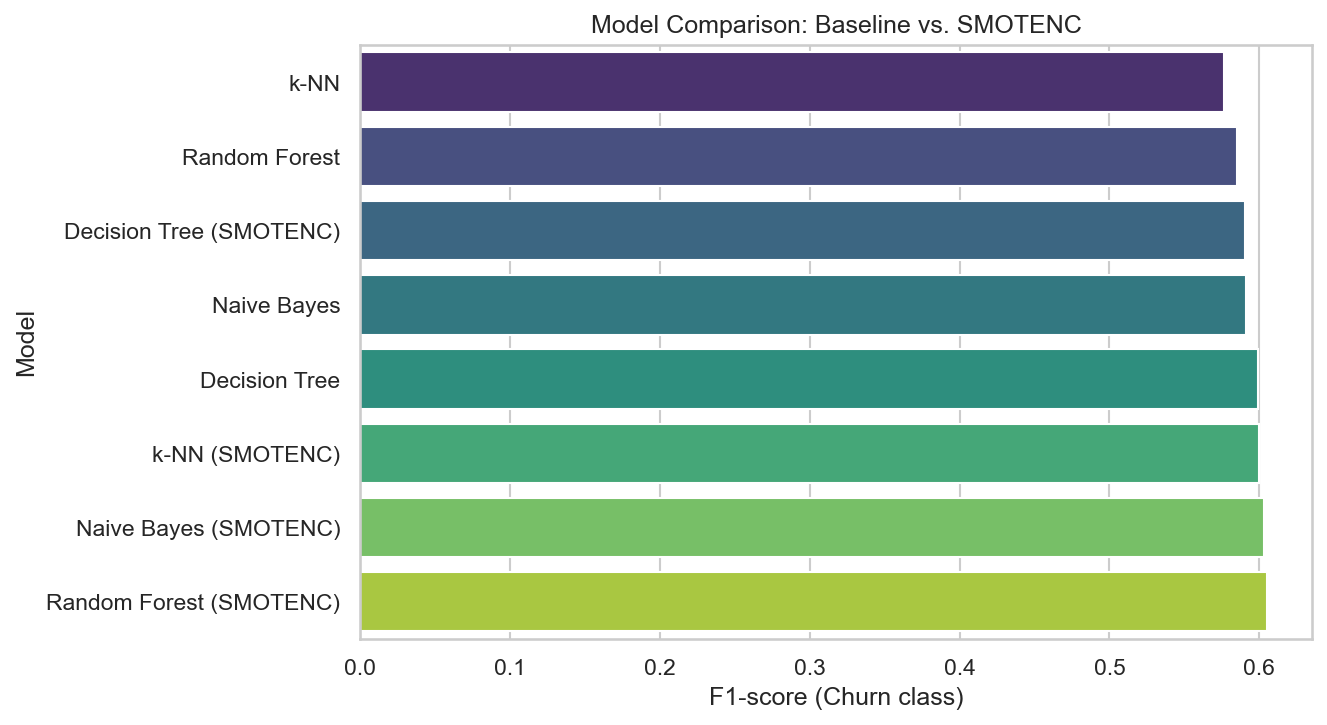
\includegraphics[width=0.48\textwidth]{figures_f1_comparison.png}
		\caption{F1-score comparison across all eight model variants.}
		\label{fig:f1comparison}
	\end{figure}
	
	\begin{figure}[htbp]
		\centering
		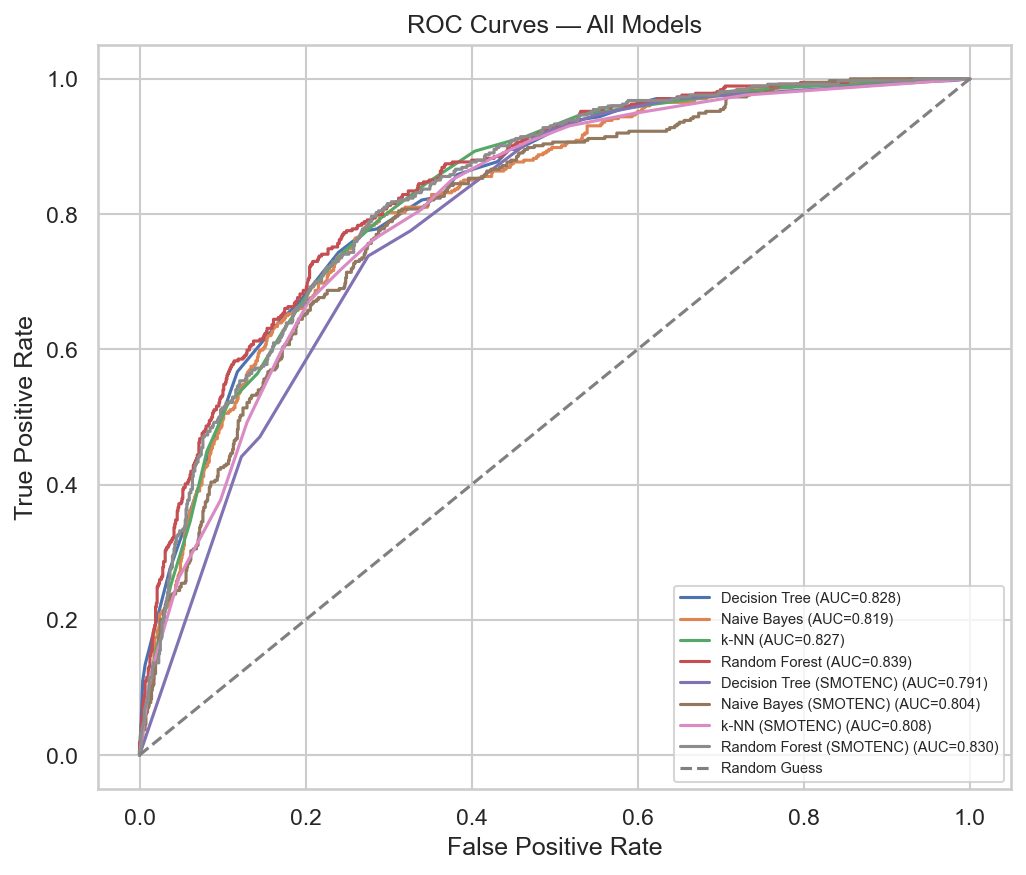
\includegraphics[width=0.48\textwidth]{figures_roc_curves.png}
		\caption{ROC curves for all eight baseline and SMOTENC-trained model variants.}
		\label{fig:roccurves}
	\end{figure}
	
	\begin{figure}[htbp]
		\centering
		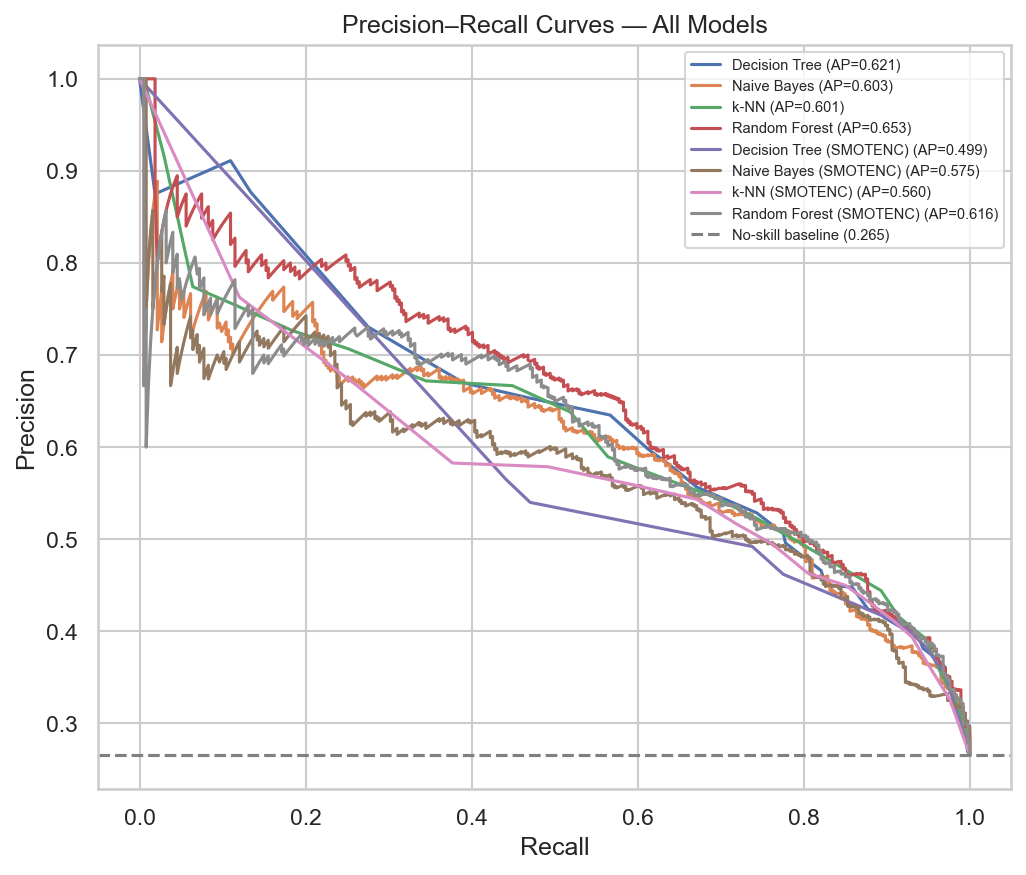
\includegraphics[width=0.48\textwidth]{figures_pr_curves.png}
		\caption{Precision--recall curves for all eight model variants.}
		\label{fig:prcurves}
	\end{figure}
	
	\begin{figure}[htbp]
		\centering
		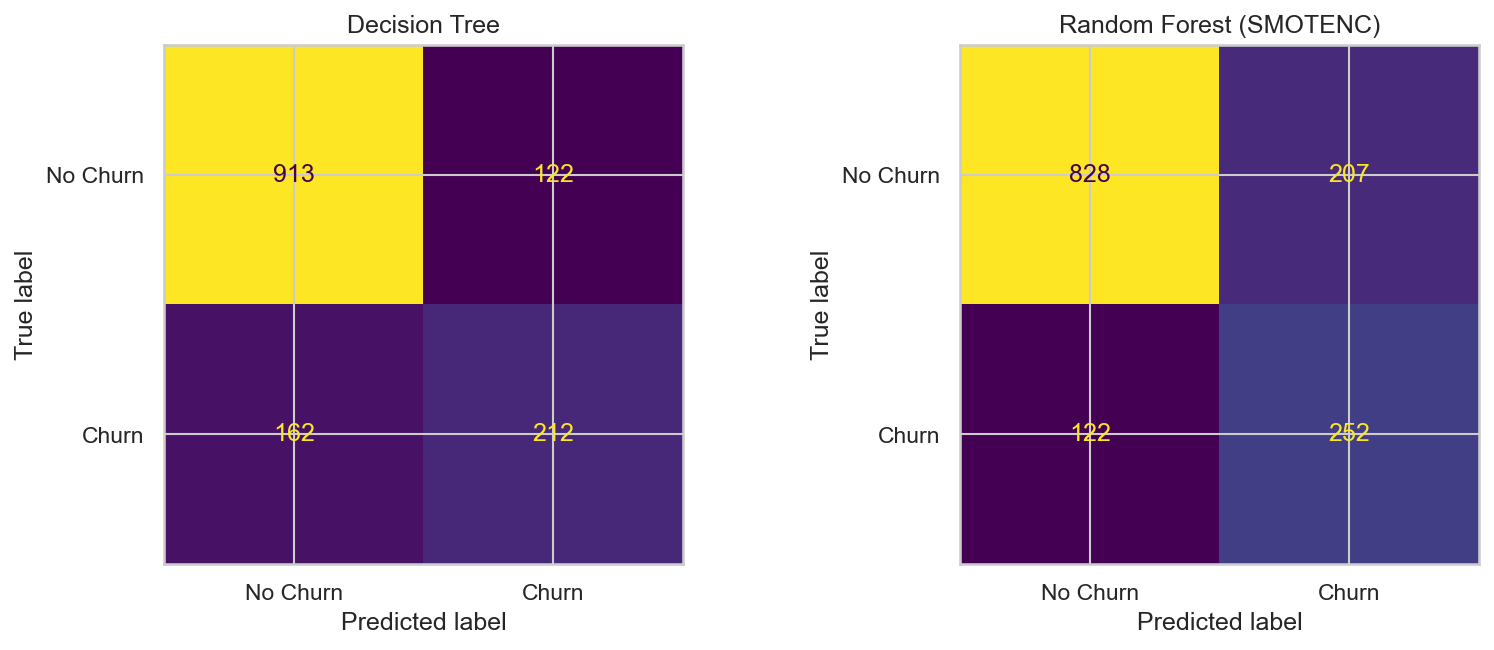
\includegraphics[width=0.48\textwidth]{figures_confusion_matrices.png}
		\caption{Confusion matrices for the best baseline model (Decision Tree, by F1) and the best SMOTENC model (Naive Bayes, by F1).}
		\label{fig:confmatrices}
	\end{figure}
	
	\begin{figure}[htbp]
		\centering
		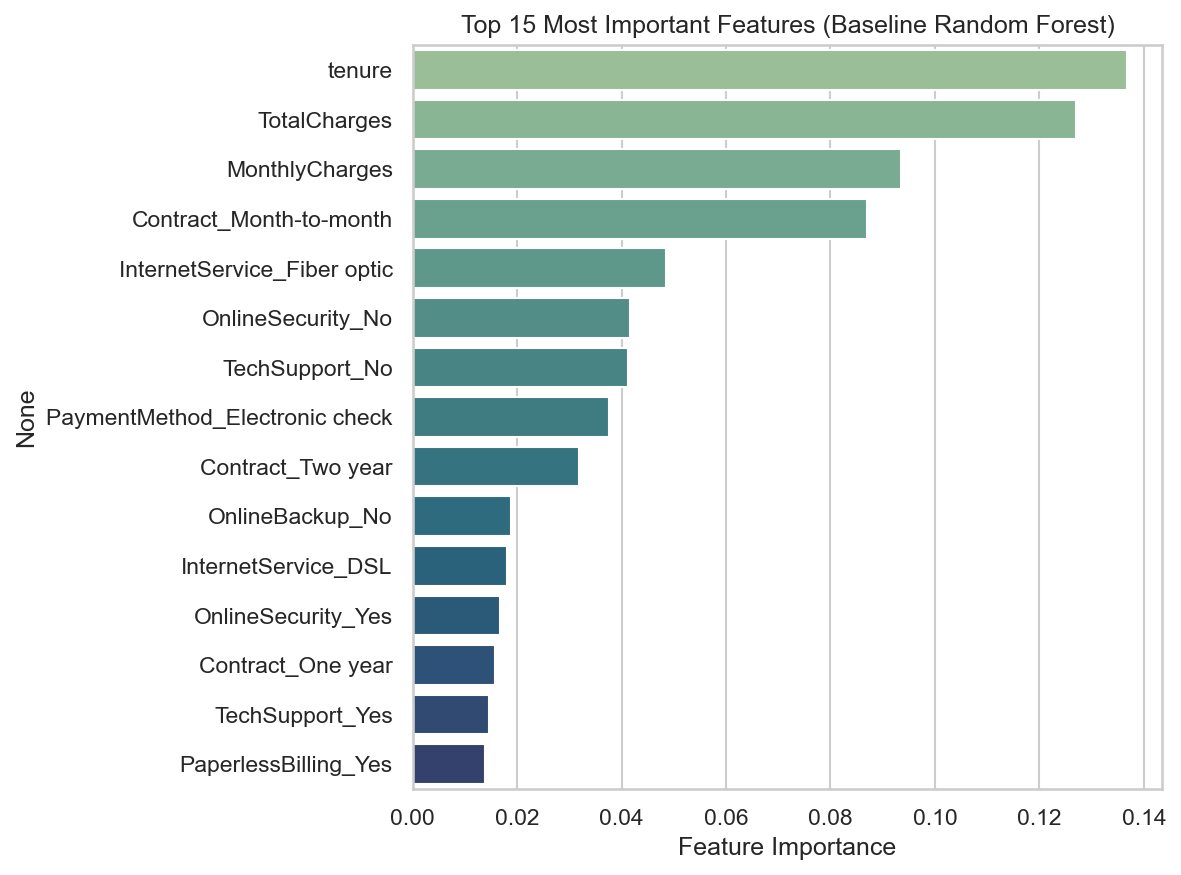
\includegraphics[width=0.48\textwidth]{figures_feature_importance.png}
		\caption{Top 15 features by importance, from the baseline Random Forest model.}
		\label{fig:featimportance}
	\end{figure}
	
	\subsection{Comparison of Approaches}
	The baseline Random Forest achieved the highest accuracy (80.3\%), ROC-AUC (0.839), and PR-AUC (0.653). Its precision was also the highest (66.2\%), but its churn recall was only 52.4\%, so it missed almost half of the actual churners. Baseline Naive Bayes showed the opposite behavior: it achieved the highest recall (81.0\%) but only 46.5\% precision. The baseline Decision Tree produced the highest baseline F1-score (0.599), balancing 63.5\% precision with 56.7\% recall.
	
	SMOTENC increased recall for Decision Tree, k-NN, and Random Forest, while Naive Bayes already had very high baseline recall and decreased slightly from 81.0\% to 77.8\%. In each algorithm family, the SMOTENC variant traded some accuracy or precision for higher minority-class sensitivity. Naive Bayes with SMOTENC achieved the highest F1-score (0.602), while Random Forest with SMOTENC was nearly tied at 0.601 and offered higher precision (54.4\% versus 49.2\%). The small F1 difference means that a practical selection should be based on retention costs rather than ranking alone: Naive Bayes with SMOTENC favors catching more churners, whereas Random Forest with SMOTENC produces fewer false alarms. If probability ranking or minimizing unnecessary interventions is more important, the baseline Random Forest remains the strongest option because of its superior ROC-AUC, PR-AUC, and precision.
	
	\section{Discussion}
	\label{sec:discussion}
	
	\textit{Best-performing method.} No single algorithm dominated every metric. Random Forest's ensemble reduced the variance of a single Decision Tree and produced the strongest baseline ranking performance, as shown by both ROC-AUC and PR-AUC. However, using the default 0.5 decision threshold, it predicted the minority class conservatively and therefore had modest churn recall. SMOTENC shifted the Random Forest toward higher recall, although precision declined. Naive Bayes with SMOTENC achieved the highest F1-score, but its lead over Random Forest with SMOTENC was only 0.001. This difference is too small to justify a deployment decision by itself. A retention team should instead choose between these models using the relative business cost of a missed churner and an unnecessary offer.
	
	\textit{Limitations.} This study is based on a single dataset from one fictional telecom provider, so the results may not generalize to companies with different customer bases, pricing structures, or markets. Hyperparameter search was limited to small grids for tractability rather than an exhaustive or nested search. The final test set was used only after model selection, but a separate temporal or external validation set was unavailable, so performance on genuinely future customers remains unknown. SMOTENC avoids invalid interpolation across categorical codes, but its synthetic minority examples still depend on local patterns in the observed churners and may not represent all future churn behavior. Finally, the models were compared at the default 0.5 threshold rather than thresholds optimized for a known business cost.
	
	\textit{Surprising findings.} Naive Bayes' strong baseline recall was somewhat unexpected given its restrictive assumption of conditional independence between features -- an assumption clearly violated here, since several one-hot encoded service attributes are correlated (e.g., a customer without internet service will have ``No internet service'' recorded across several related columns simultaneously). This suggests that even with a misspecified independence assumption, Naive Bayes' probabilistic scoring can still be useful as a high-recall screening step, for example to generate an initial candidate list of at-risk customers that a more precise model or human reviewer then narrows down.
	
	\textit{Effect of data-quality issues.} The hidden \texttt{TotalCharges} blank-string issue (Section~\ref{sec:methodology}) affected only 11 of 7{,}043 records (0.16\%) and therefore had little direct effect on aggregate performance. Its importance is methodological: a standard null count did not reveal the problem. The class imbalance, by contrast, substantially affected the evaluation. It produced the accuracy--recall trade-off between most baseline and SMOTENC variants and explains why a metric such as PR-AUC is more informative than accuracy alone.
	
	\textit{Ethical implications.} As noted in Section~\ref{sec:dataset}, demographic attributes were not among the dominant predictors identified by the Random Forest (Fig.~\ref{fig:featimportance}); the model instead relies mainly on tenure, billing, and service/contract attributes. This is a reassuring sign for fairness, but not a guarantee, since attributes like \texttt{Contract} and \texttt{PaymentMethod} could still correlate with protected characteristics indirectly. A production deployment of this model should include periodic subgroup performance audits (e.g., comparing recall across demographic groups) before being used to allocate retention resources.
	
	\section{Conclusion and Future Work}
	\label{sec:conclusion}
	
	This project compared Decision Tree, Gaussian Naive Bayes, k-NN, and Random Forest classifiers for predicting customer churn, with both baseline and SMOTENC training pipelines. The baseline Random Forest achieved the highest accuracy (80.3\%), precision (66.2\%), ROC-AUC (0.839), and PR-AUC (0.653). Naive Bayes with SMOTENC achieved the highest F1-score (0.602) and 77.8\% recall, while Random Forest with SMOTENC achieved an almost identical F1-score (0.601) with higher precision. The main practical conclusion is therefore not that one model is universally best. A high-recall retention campaign could prefer Naive Bayes with SMOTENC, while a campaign seeking to reduce unnecessary offers or rank customers reliably could prefer Random Forest. The Random Forest feature-importance analysis identifies which variables most influenced its predictions, but it does not establish the direction of those effects or a causal relationship with churn.
	
	With more time, this project could be extended with (i) a broader hyperparameter search and nested cross-validation, (ii) additional algorithms such as Logistic Regression, Gradient Boosting, and XGBoost~\cite{b1}, (iii) alternatives to SMOTENC such as class weighting or cost-sensitive learning, and (iv) threshold selection based on the actual costs of false positives and false negatives. Future work could also test generalizability on data from another provider or time period, add customer-service interaction features, inspect directional effects with methods such as partial dependence or SHAP, and audit error rates across demographic groups before deployment.
	
	\section*{AI Tool Use and Originality Declaration}
	\label{sec:ai_declaration}
	
	\textbf{[Draft -- must be reviewed and completed truthfully by the student before submission; see note below the table.]}
	
	AI-assisted tools were used only for limited support, such as identifying and helping to verify literature-search candidates, drafting report structure and language, concept clarification, and/or LaTeX formatting. The project idea, methodology choices, experiments, analysis, interpretation of results, and final report wording were reviewed, verified, and finalized by the student. The student accepts full responsibility for the accuracy, originality, reproducibility, and integrity of the submitted work.
	
	\begin{table}[htbp]
		\caption{AI Use Disclosure Summary (Draft -- adjust to reflect actual use)}
		\label{tab:ai_use}
		\centering
		\footnotesize
		\begin{tabular}{|p{0.35\linewidth}|c|p{0.38\linewidth}|}
			\hline
			\textbf{Project Stage} & \textbf{Level} & \textbf{Brief Description} \\
			\hline
			Conceptualization and idea generation & [0--6] & AI suggested candidate topics/datasets; final choice and rationale by student. \\
			\hline
			Literature search and synthesis & [0--6] & AI located candidate papers; student must independently read and verify each source before submission. \\
			\hline
			Methodology, coding, and analysis & [0--6] & AI drafted the preprocessing/modeling notebooks and ran the experiments; student must review, re-run, and understand every step before submission. \\
			\hline
			Writing, editing, and LaTeX formatting & [0--6] & AI drafted section text and formatting; student must rewrite/review in their own words. \\
			\hline
			Interpretation, discussion, and conclusion & [0--6] & AI drafted an initial interpretation of the real results; student must rewrite this as their own analysis and judgment. \\
			\hline
		\end{tabular}
	\end{table}
	
	\begin{thebibliography}{00}
		
		\bibitem{b1} A.~K.~Ahmad, A.~Jafar, and K.~Aljoumaa, ``Customer churn prediction in telecom using machine learning in big data platform,'' \textit{Journal of Big Data}, vol.~6, no.~1, p.~28, 2019.
		
		\bibitem{b2} N.~Mustafa, L.~Sook Ling, and S.~F.~Abdul Razak, ``Customer churn prediction for telecommunication industry: A Malaysian case study,'' \textit{F1000Research}, vol.~10, p.~1274, 2021.
		
		\bibitem{b3} J.~K.~Sana, M.~Z.~Abedin, M.~S.~Rahman, and M.~S.~Rahman, ``A novel customer churn prediction model for the telecommunication industry using data transformation methods and feature selection,'' \textit{PLOS ONE}, vol.~17, no.~12, p.~e0278095, 2022.
		
		\bibitem{b4} N.~V.~Chawla, K.~W.~Bowyer, L.~O.~Hall, and W.~P.~Kegelmeyer, ``SMOTE: Synthetic minority over-sampling technique,'' \textit{Journal of Artificial Intelligence Research}, vol.~16, pp.~321--357, 2002.
		
	\end{thebibliography}
	
	\newpage	
	\appendix
	
	\section{Code Repository}
	\label{app:code}
	
	Full source code is available at: \url{https://github.com/[yourusername]/[project-repo]} \textbf{[Placeholder -- update once the repository is created.]}
	
	\begin{lstlisting}[caption={Data Loading and Cleaning (excerpt)}, label={lst:preprocess}]
import pandas as pd

df = pd.read_csv(
    'data/WA_Fn-UseC_-Telco-Customer-Churn.csv'
)

# TotalCharges is stored as text; blanks correspond
# to tenure == 0 (new, unbilled customers)
df['TotalCharges'] = pd.to_numeric(
    df['TotalCharges'], errors='coerce'
).fillna(0)

df = df.drop(columns=['customerID'])
df['SeniorCitizen'] = df['SeniorCitizen'].map(
    {0: 'No', 1: 'Yes'}
)
df['Churn_binary'] = df['Churn'].map({'No': 0, 'Yes': 1})
	\end{lstlisting}
	
	\section{AI Prompt and Verification Log (If Applicable)}
	\label{app:ai_log}
	
	\textbf{[Placeholder -- if required by the instructor, summarize key prompts used, their purpose, and how outputs were verified.]}
	
	\section{Additional Figures and Tables}
	\label{app:additional}
	
	The main results table, F1-score comparison, ROC curves, precision--recall curves, confusion matrices, and feature-importance plot are included in Section~\ref{sec:results}. Table~\ref{tab:hyperparams} reports the best hyperparameters selected via stratified 5-fold cross-validation (optimizing F1-score). Baseline and SMOTENC variants were tuned independently.
	
	\begin{table}[htbp]
		\caption{Selected Hyperparameters (5-fold CV, optimizing F1)}
		\label{tab:hyperparams}
		\begin{center}
			\footnotesize
			\resizebox{\columnwidth}{!}{%
			\begin{tabular}{|l|l|c|}
				\hline
				\textbf{Model} & \textbf{Best Hyperparameters} & \textbf{CV F1} \\
				\hline
				Decision Tree & max\_depth=5, min\_samples\_leaf=10 & 0.565 \\
				\hline
				Naive Bayes & var\_smoothing=1e-7 & 0.599 \\
				\hline
				k-NN & n\_neighbors=21 & 0.591 \\
				\hline
				Random Forest & n\_estimators=200, max\_depth=10 & 0.578 \\
				\hline
				Decision Tree (SMOTENC) & max\_depth=3, min\_samples\_leaf=1 & 0.593 \\
				\hline
				Naive Bayes (SMOTENC) & var\_smoothing=1e-9 & 0.612 \\
				\hline
				k-NN (SMOTENC) & n\_neighbors=15 & 0.608 \\
				\hline
				Random Forest (SMOTENC) & n\_estimators=200, max\_depth=10 & 0.626 \\
				\hline
			\end{tabular}}
		\end{center}
	\end{table}
	
\end{document}
